\documentclass{article}
\usepackage{amsmath}

\usepackage{graphicx}

\usepackage{listings}
\usepackage{color}
\definecolor{dkgreen}{rgb}{0,0.6,0}
\definecolor{gray}{rgb}{0.5,0.5,0.5}
\definecolor{mauve}{rgb}{0.58,0,0.82}
\lstset{frame=tb,
  language=R,
  aboveskip=3mm,
  belowskip=3mm,
  showstringspaces=false,
  columns=flexible,
  basicstyle={\small\ttfamily},
  numbers=none,
  numberstyle=\tiny\color{gray},
  keywordstyle=\color{blue},
  commentstyle=\color{dkgreen},
  stringstyle=\color{mauve},
  breaklines=false,
  breakatwhitespace=true,
  tabsize=3
}

\title{SDS385 Fall '16: Statistical Models For Big Data\\Exercises 01 - Generalized linear models}
\author{Matteo Vestrucci}
\date{September 1st 2016}
\begin{document}
\maketitle
\bigskip\bigskip\bigskip

\subsubsection*{A)}

The negative log-likelihood can be rewritten like this:

\begin{align*}
l(\beta)&=-\log\left\lbrace\prod_{i=1}^N p(y_i|\beta)\right\rbrace\\
		&=-\log\left[\prod_{i=1}^N \binom{m_i}{y_i}w_i^{y_i}(1-w_i)^{m_i-y_i}\right]\\
		&= c-\sum_{i=1}^N y_i \log(w_i)-\sum_{i=1}^N m_i \log(1-w_i)+\sum_{i=1}^N y_i \log(1-w_i)\\
		&= c-\sum_{i=1}^N y_i \log\left(\frac{w_i}{1-w_i}\right)-\sum_{i=1}^N m_i \log(1-w_i)\\
		&= c-\sum_{i=1}^N y_i \log\left(\frac{1}{e^{-x_i^T\beta}}\right)-\sum_{i=1}^N m_i \log\left(\frac{e^{-x_i^T\beta}}{1+e^{-x_i^T\beta}}\right)\\
		&= c-\sum_{i=1}^N y_i x_i^T\beta+\sum_{i=1}^N m_i x_i^T\beta+\sum_{i=1}^N m_i \log(1+e^{-x_i^T\beta})\\
		&\approx\sum_{i=1}^N (m_i-y_i) x_i^T\beta+\sum_{i=1}^N m_i \log(1+e^{-x_i^T\beta})
\end{align*}

\newpage

Its gradient is:

\begin{align*}
\nabla l(\beta)&=\nabla\left(\sum_{i=1}^N (m_i-y_i) x_i^T\beta+\sum_{i=1}^N m_i \log(1+e^{-x_i^T\beta})\right)\\
				&=\sum_{i=1}^N (m_i-y_i) x_i+\sum_{i=1}^N m_i w_i e^{-x_i^T\beta}(-x_i)\\
				&=\sum_{i=1}^N m_i x_i-\sum_{i=1}^N y_i x_i-\sum_{i=1}^N m_i (1-w_i) x_i\\
				&=-\sum_{i=1}^N y_i x_i+\sum_{i=1}^N m_i w_i x_i\\
				&=\sum_{i=1}^N (m_i w_i-y_i)x_i=\sum_{i=1}^N (\hat{y}-y_i)x_i=X^TS\\
\end{align*}

where $S$ is a vector with $i$-th element $m_i w_i-y_i$.

\subsubsection*{B)}

The gradient descent updates at each step the values of our estimated $\beta$ using this formula:

\begin{equation*}
\beta_{t+1}=\beta_t-a\nabla l(\beta_t)
\end{equation*}

with $a$ being the step size. Running the code in appendix, we can obtain the following $\hat{\beta}$:\\

\begin{tabular}{ll}
c			&-0.0033014219\\
V3          &-0.0231821340\\
V4          &-0.0174151223\\
V5          &-0.1233097211\\
V6          & 0.0182791149\\
V7          &-0.0001358173\\
V8          & 0.0004527453\\
V9          & 0.0008734747\\
V10         & 0.0003869764\\
V11         &-0.0002857808\\
V12         &-0.0001459426
\end{tabular}\\

The following graph of the objective function shows us that indeed it's being decreased at each step.

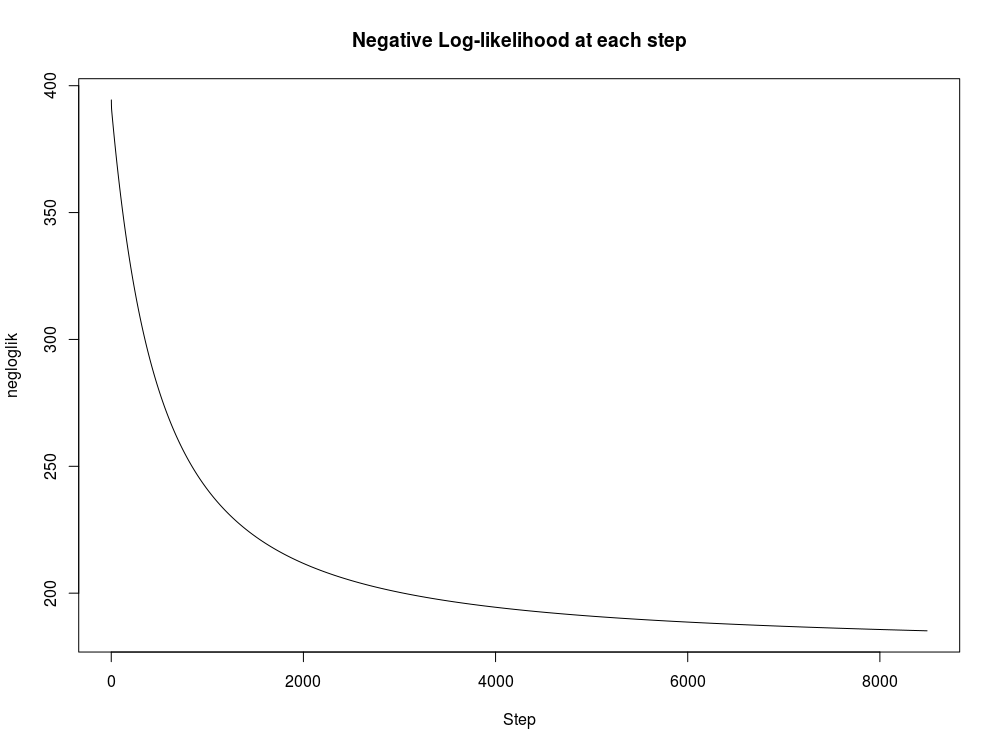
\includegraphics[width=\textwidth]{Rplot_gradient.png}

\subsubsection*{C)}

The Hessian is:

\begin{align*}
\nabla^2 l(\beta)&=\nabla \left(-\sum_{i=1}^N y_i x_i+\sum_{i=1}^N m_i w_i x_i\right)\\
				 &=\nabla \left( c+\sum_{i=1}^N m_i x_{i1}\frac{1}{1+e^{-x_i^T\beta}}\enskip,\enskip \dots \enskip,\enskip c+\sum_{i=1}^N m_i x_{iP}\frac{1}{1+e^{-x_i^T\beta}} \right)\\
				 &=\begin{bmatrix} \sum_{i=1}^N m_i x_{i1}\frac{-e^{-x_i^T\beta}}{\left(1+e^{-x_i^T\beta}\right)^2}(-x_{i1}) & \cdots & \sum_{i=1}^N m_i x_{i1}\frac{-e^{-x_i^T\beta}}{\left(1+e^{-x_i^T\beta}\right)^2}(-x_{iP}) \\ \vdots & \ddots & \vdots \\ \sum_{i=1}^N m_i x_{iP}\frac{-e^{-x_i^T\beta}}{\left(1+e^{-x_i^T\beta}\right)^2}(-x_{i1}) & \cdots & \sum_{i=1}^N m_i x_{iP}\frac{-e^{-x_i^T\beta}}{\left(1+e^{-x_i^T\beta}\right)^2}(-x_{iP}) \end{bmatrix}\\
				 &=\begin{bmatrix} \sum_{i=1}^N m_i x_{i1}x_{i1}w_i(1-w_i) & \cdots & \sum_{i=1}^N m_i x_{i1}x_{iP}w_i(1-w_i) \\ \vdots & \ddots & \vdots \\ \sum_{i=1}^N m_i x_{iP}x_{i1}w_i(1-w_i) & \cdots & \sum_{i=1}^N m_i x_{iP}x_{iP}w_i(1-w_i) \end{bmatrix}=X^TDX
\end{align*}\\

where $D$ is a diagonal matrix with $ii$-th element $m_i w_i (1-w_i)$. Notice that all the values on the diagonal are positive: this means that the Hessian is defined positive and that our objective function is convex. Then, considering that we can ignore the constant values adding and subtracting them as we need, we can obtain the requested result like this:

\begin{align*}
q_l(\beta,\beta_0)&=l(\beta_0)+\nabla(\beta_0)^T(\beta-\beta_0)+\frac{1}{2}(\beta-\beta_0)^t\nabla^2(\beta_0)(\beta-\beta_0)\\
				  &=c+S^TX(\beta-\beta_0)+\frac{1}{2}(\beta-\beta_0)^TX^TDX(\beta-\beta_0)\\				  
				  &=c+S^TX\beta+\frac{1}{2}\beta^TX^TDX\beta-\frac{1}{2}\beta^TX^TDX\beta_0-\frac{1}{2}\beta_0^TX^TDX\beta_0\\
				  &=c-(\beta_0^TX^TD-S^T)X\beta+\frac{1}{2}\beta^TX^TDX\beta\\
				  &=c-(\beta_0^TX^TD-S^T)D^{-1}DX\beta+\frac{1}{2}\beta^TX^TDX\beta\\
				  &\qquad+\frac{1}{2}(\beta_0^TX^TD-S^T)D^{-1}DD^{-1}(\beta_0^TX^TD-S^T)^T\\
				  &=c+\frac{1}{2}[D^{-1}(\beta_0^TX^TD-S^T)^T-X\beta]^TD[(D^{-1}(\beta_0^TX^TD-S^T)^T-X\beta]\\
				  &=c+\frac{1}{2}[(X\beta_0-D^{-1}S)-X\beta]^TD[(X\beta_0-D^{-1}S)-X\beta]\\
 				  &=c+\frac{1}{2}[Z-X\beta]^TW[Z-X\beta]
\end{align*}\\

where $Z$ is the vector $X\beta_0-D^{-1}S$ and where $W$ is the matrix $D$.

\subsubsection*{D)}

The newton's method updates at each step the values of our estimated $\beta$ using this formula:

\begin{equation*}
\beta_{t+1}=\beta_t-[\nabla^2 l(\beta_t)]^{-1}\nabla l(\beta_t)
\end{equation*}

Running the code in appendix, we can obtain the following $\hat{\beta}$:\\

\begin{tabular}{ll}
c			 &-7.35951761\\
V3           &-2.04930490\\
V4           & 0.38473434\\
V5           &-0.07151042\\
V6           & 0.03979620\\
V7           &76.43227376\\
V8           &-1.46242225\\
V9           & 8.46869976\\
V10          &66.82175685\\
V11          &16.27824232\\
V12          &-68.33702689
\end{tabular}\\

The following graph of the objective function shows us that indeed it's being decreased at each step.

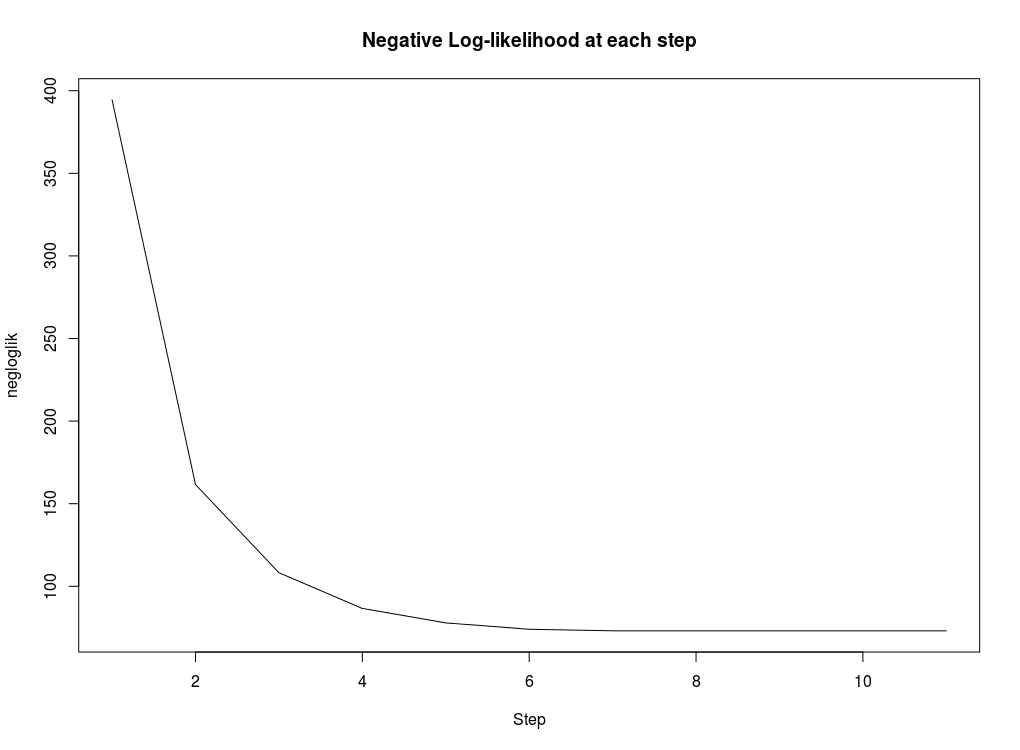
\includegraphics[width=\textwidth]{Rplot_newton.png}

\subsubsection*{CODE)}

\begin{lstlisting}
library(Matrix)

negloglikelihood<-function(m,y,X,beta){
  total<-0
  N<-length(y)
  for(i in 1:N) total<-total+(m[i]-y[i])*t(X[i,])%*%beta+m[i]*log(1+exp(-t(X[i,])%*%beta))
  return(total)
}

gradient_negloglik<-function(m,y,X,beta){
  w<-1/(1+exp(-X%*%beta))
  S<-m*w-y
  grad<-t(X)%*%S
  return(grad)
}

gradient_descent<-function(m,y,X,beta0,stepsize,maxstepnumber,
                           accuracy_obj_fun,accuracy_beta_val){
  negloglik<-numeric(maxstepnumber)
  negloglik[1]<-negloglikelihood(m,y,X,beta0)
  gradient<-gradient_negloglik(m,y,X,beta0)
  diff_beta_val<-accuracy_beta_val+1
  diff_obj_fun<-accuracy_obj_fun+1
  i<-1
  while(!(i==maxstepnumber)&&
        ((accuracy_beta_val<diff_beta_val)||
        (accuracy_obj_fun<diff_obj_fun))){
    i<-i+1
    beta1<-beta0-stepsize*gradient
    diff_beta_val<-sum(abs(beta0-beta1))
    beta0<-beta1
    negloglik[i]<-negloglikelihood(m,y,X,beta0)
    diff_obj_fun<-negloglik[i-1]-negloglik[i]
    gradient<-gradient_negloglik(m,y,X,beta0)
  }
  return(list(betahat=beta0,negloglik=negloglik,step=i))
}

data_wdbc<-read.csv("./wdbc.csv", header=FALSE)
X<-as.matrix(cbind(rep(1,569),data_wdbc[,3:12]))
y<-data_wdbc[,2]
y<-as.numeric(y=="M")
m<-rep(1,569)

beta0<-rep(0,11)
stepsize<-2/10^8
maxstepnumber<-10000
accuracy_obj_fun<-0.001
accuracy_beta_val<-0.00001
result_grad_desc<-gradient_descent(m,y,X,beta0,stepsize,maxstepnumber,
                                   accuracy_obj_fun,accuracy_beta_val)

result_grad_desc$betahat
plot(result_grad_desc$negloglik[1:result_grad_desc$step],
     main = "Negative Log-likelihood at each step",
     xlab="Step",ylab="negloglik",type="l")

hessian_negloglik<-function(m,y,X,beta){
  w<-as.vector(1/(1+exp(-X%*%beta)))
  D<-diag(m*w*(1-w))
  hes<-t(X)%*%D%*%X
  return(hes)
}

newton_descent<-function(m,y,X,beta0,maxstepnumber,
                         accuracy_obj_fun,accuracy_beta_val){
  negloglik<-numeric(maxstepnumber)
  negloglik[1]<-negloglikelihood(m,y,X,beta0)
  gradient<-gradient_negloglik(m,y,X,beta0)
  hessian<-hessian_negloglik(m,y,X,beta0)
  diff_beta_val<-accuracy_beta_val+1
  diff_obj_fun<-accuracy_obj_fun+1
  i<-1
  while(!(i==maxstepnumber)&&
        ((accuracy_beta_val<diff_beta_val)||
        (accuracy_obj_fun<diff_obj_fun))){
    i<-i+1
    beta1<-beta0-solve(hessian,gradient)
    diff_beta_val<-sum(abs(beta0-beta1))
    beta0<-beta1
    negloglik[i]<-negloglikelihood(m,y,X,beta0)
    diff_obj_fun<-negloglik[i-1]-negloglik[i]
    gradient<-gradient_negloglik(m,y,X,beta0)
    hessian<-hessian_negloglik(m,y,X,beta0)
  }
  return(list(betahat=beta0,negloglik=negloglik,step=i))
}

result_newton_desc<-newton_descent(m,y,X,beta0,maxstepnumber,
                                   accuracy_obj_fun,accuracy_beta_val)

result_newton_desc$betahat
plot(result_newton_desc$negloglik[1:result_newton_desc$step],
     main = "Negative Log-likelihood at each step",
     xlab="Step",ylab="negloglik",type="l")
\end{lstlisting}

\end{document}